A rotation matrix $^a_bR$ is an orthonormal matrix ($R^{-1}=R^T$) describing the rotation between two right-handed coordinate frames $\Psi_a$ and $\Psi_b$ such that any vector $^bv$ (including $\Psi_b$ coordinate axes) given in the $\Psi_b$ frame can be "rotated" into $\Psi_a$ coordinates by the operation
\begin{equation}
^av =\, ^a_bR \,\,^bv
\end{equation}
Note that the matrix $^a_bR$ can also be seen as the rotation required of the frame $\Psi_a$ for it to coincide with $\Psi_b$.
Rotation of the frame $\Psi_a$ with an angle $\theta$ counterclockwise about a single axis (equal to clockwise "rotation" of the any vector in $\Psi_b$) correspond to the rotation matrices
\begin{small}
\begin{equation}
^a_bR_x(\theta) = 
\begin{bmatrix}
1 & 0 & 0\\
0 & \cos\theta & -\sin\theta\\
0 & \sin\theta & \cos\theta
\end{bmatrix} 
\qquad
^a_bR_y(\theta) = 
\begin{bmatrix}
\cos\theta & 0 & \sin\theta \\
0 & 1 & 0\\
-\sin\theta & 0 & \cos\theta
\end{bmatrix}
\qquad
^a_bR_z(\theta) = 
\begin{bmatrix}
\cos\theta & -\sin\theta & 0\\
\sin\theta & \cos\theta & 0\\
0 & 0 & 1
\end{bmatrix}
\label{eq:RxRyRz}
\end{equation}
\end{small}
A sequence of rotations, transforming the vector $^cv$ given in the $\Psi_c$ frame to $\Psi_a$ coordinates, is implemented as
\begin{equation}
^av = \underbrace{^a_bR \,\, ^b_cR}_{^a_cR} \,\,^cv 
\end{equation}

The translation of the origin from the coordinate system $\Psi_a$ to $\Psi_b$ can be described by the position vector $^a_bp$, which is a vector given in the $\Psi_a$ coordinate frame.
The relative configuration of two coordinate frames is their relative position and orientation, which can be expressed expressed by a homogeneous matrix
\begin{equation}
^a_bH = 
\begin{bmatrix}
^a_bR & ^a_bp\\
0 & 1
\end{bmatrix}
\end{equation}
The inverse of a configuration matrix is
\begin{equation}
^a_bH^{-1} = 
\begin{bmatrix}
^a_bR^T & -^a_bR^T\,\,^a_bp\\
0 & 1
\end{bmatrix}
\end{equation}
A sequence of configurations is implemented as
\begin{equation}
^a_nH =\,\, ^a_bH \,\, ^b_cH \,\,...\,\, ^m_nH = 
\begin{bmatrix}
^a_bR \,\, ^b_cR \,\,...\,\, ^l_mR \,\,^m_nR & ^a_bp + ^a_bR \,\, ^b_cp + ... + (^a_bR\,\, ^b_cR \,\,...\,\, ^l_mR \,\, ^m_np )\\
0 & 1
\end{bmatrix}
\end{equation}
where each matrix $H$ is a function of a rotation angle $\theta$ and a translation distance, which may be functions of time.


\section{Existing Kinematics for the AAU da Vinci Robot}
The position of the end-effector (the tip of the instrument) given in an inertial frame can be described as a sequence of joint rotations of the robot and the instrument, and translation from the inertial origin via the fixed-length links and the slide of the instrument.

A coordinate frame is defined for each degree of freedom, with origin on the axis of rotation. A set of coordinate frames and transformation matrices between the frames are given according to the \gls{ros} \texttt{xacro} files \texttt{tower}, \texttt{p4\_arm}, \texttt{remote\_center\_manipulator} and \texttt{needle\_driver}.

\begin{figure}[htbp]
\vspace*{-10mm}
\hspace{-10mm}
\subbottom[Coordinate frames for the joints on the robot arm.]{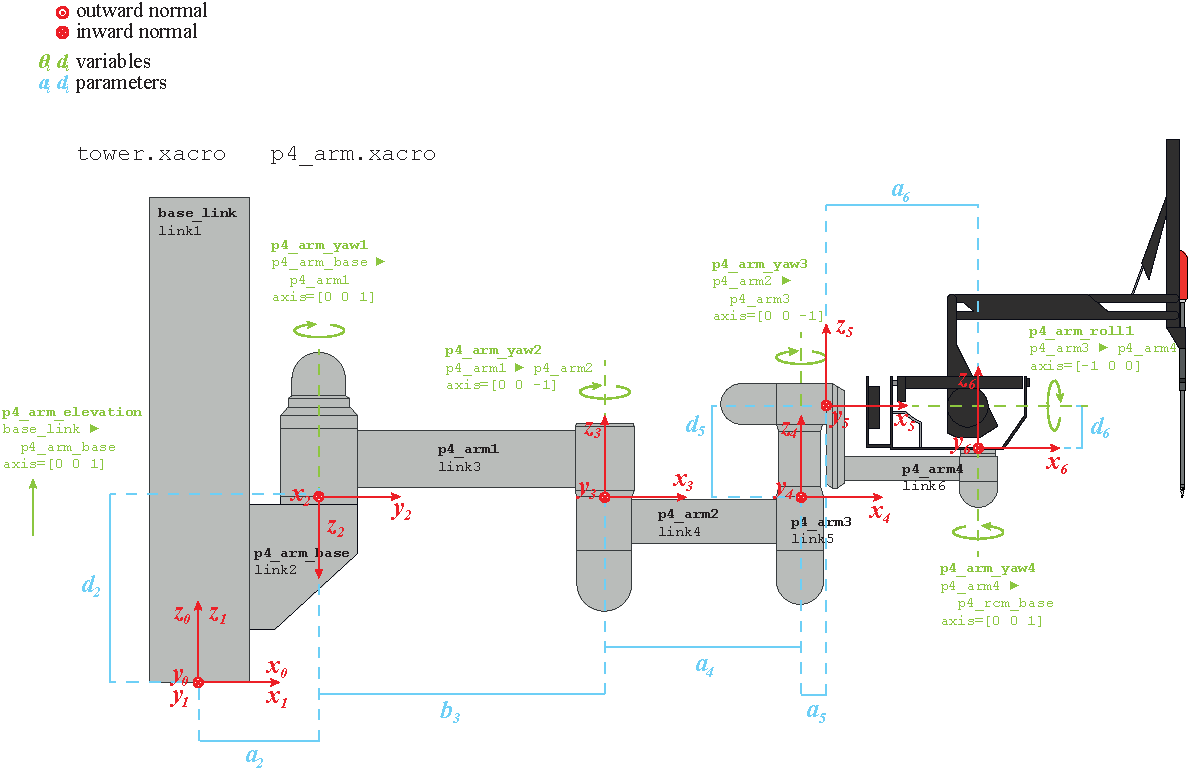
\includegraphics[width=1.1\textwidth]{p4_arm_xacro_frames.pdf}\label{fig:p4_arm_xacro_frames}}%
\vspace{5mm}\\
\hspace*{-15mm}
\subbottom[Coordinate frames for the joints on the robot hand and instrument.]{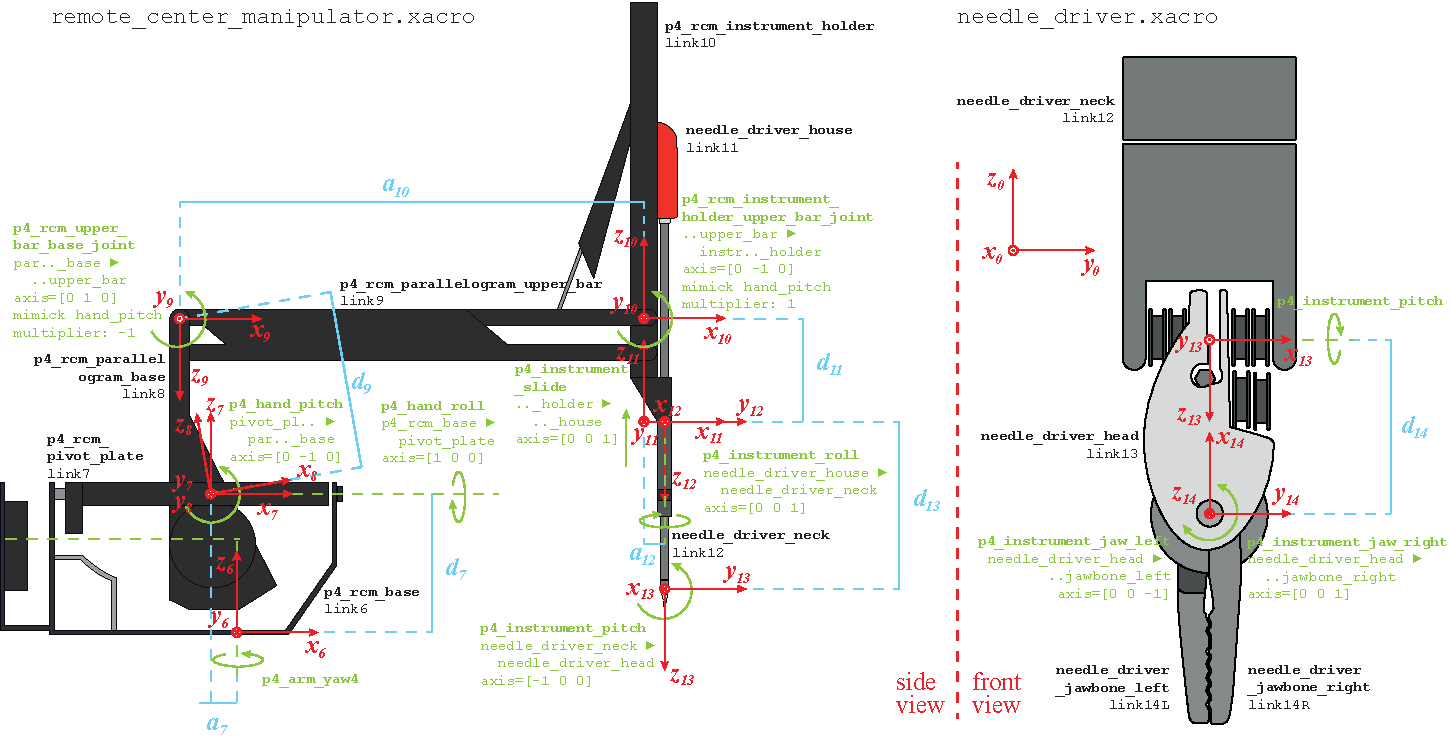
\includegraphics[width=1.15\textwidth]{p4_hand_xacro_frames.pdf}\label{fig:p4_hand_xacro_frames}}%
\caption{Orientation and position of coordinate frames $\Psi_0$, $\Psi_b$, $\Psi_1$, ..., $\Psi_{14}$ according to the \gls{ros} \texttt{xacro} files.}
\label{fig:robot_xacro_frames}
\end{figure}

The position and orientation of the $i$th coordinate frame is given as a transformation matrix from the $i-1$th frame, where fixed distances and rotations are measured along/about the axes of the $i-1$th frame while free distances and rotations are measured along/about the axes of the $i$th frame. The parameters and variables shown in \autoref{fig:robot_xacro_frames} are given in \autoref{tab:xacro_param}.

\vspace{2mm}
\begin{table}[htbp]
\small
\centering
	\begin{tabular}{r | rrr c c l}\hline
		frame  & $a$ [m] & $b$ [m] & $d$ [m] & fixed rot. $\alpha$ [rad] & free rot. $\theta$ [rad] & name\\\hline
		1 & 0 & 0 & $d_1^*$ & $I$ & $I$ & \texttt{elevation}\\
		2 & 0.186 & 0 & 0.554 & $R_z(\pi/2)R_x(\pi)$ & $R_z(\theta_2^*)$ & \texttt{arm\_yaw1} \\
		3 & 0 & 0.583 & 0 & $R_z(\pi/2)R_x(-\pi)$ & $R_z(-\theta_3^*)$ & \texttt{arm\_yaw2} \\
		4 & 0.479 & 0 & -0.001 & $I$ & $R_z(-\theta_4^*)$ & \texttt{arm\_yaw3} \\
		5 & 0.057 & 0 & 0.198 & $I$ & $R_x(-\theta_5^*)$ & \texttt{arm\_roll1} \\
		6 & 0.352 & 0 & -0.117 & $I$ & $R_z(\theta_6^*)$ & \texttt{arm\_yaw4} \\
		7 & -0.042 & 0 & 0.161 & $I$ & $R_x(\theta_7^*)$ & \texttt{hand\_roll} \\
		8 & 0 & 0 & 0 & $R_y(-0.288)$ & $R_y(-\theta_8^*)$ & \texttt{hand\_pitch} \\
		9 & 0.011 & 0 & 0.186 & $R_y(0.288)R_x(\pi)$ & $R_y(-\theta_8)$ & \texttt{upper\_bar} \\
		10 & 0.520 & 0 & 0 & $R_x(\pi)$ & $R_y(-\theta_8)$ & \texttt{instrument\_holder} \\
		11 & 0 & 0 & -0.120 + $d_{11}^*$ & $I$ & $I$ & \texttt{instrument\_slide} \\
		12 & 0.052 & 0 & 0 & $R_z(\pi/2)R_x(\pi)$ & $R_z(\theta_{12}^*)$ & \texttt{instrument\_roll} \\
		13 & 0 & 0 & 0.177 & $I$ & $R_x(-\theta_{13}^*)$ & \texttt{instrument\_pitch} \\
		14L & 0 & 0 & 0.009 & $R_y(\pi/2)R_x(\pi/2)$ & $R_z(-\theta_{14L}^*)$ & \texttt{instrument\_jaw\_left} \\
		14R & 0 & 0 & 0.009 & $R_y(\pi/2)R_x(\pi/2)$ & $R_z(\theta_{14R}^*)$ & \texttt{instrument\_jaw\_right} \\
	\end{tabular}
	\caption{Variables (marked with $^*$) and parameters for the robot in \autoref{fig:robot_xacro_frames}. $I$ is the identity matrix (no rotation). Recent measures indicate that $d_2=0.812$, $a_2=0.198$, $a_4=0.435$, $\alpha_8=R_y(-0.07)$, $\alpha_9=R_y(0.07)R_x(\pi)$, $a_9=0$ and $d_\text{11,fixed}=0.188$ ($\Rightarrow$ $d_{12}=0.472$).}
	\label{tab:xacro_param}
\end{table}


I.e. according to \autoref{tab:xacro_param}, the transformation between frame 1 and 2 is given as:
\begin{equation}
^1_2H = 
\begin{bmatrix}
R_z(\pi/2)R_x(\pi)R_z(\theta_2^*) & p_2\\
0 & 1
\end{bmatrix}, \qquad\qquad
p_2 = [0.186 \quad 0 \quad 0.554]^T
\end{equation}

The physical, low level controller and \gls{ros} limits for each of the variables are given in \autoref{tab:var_limits}

\vspace{2mm}
\begin{table}[htbp]
\small
\hspace*{-9mm}
%\begin{tabular}{l | cccccc}
%limits & $d_1^*$ & $\theta_2^*$ & $\theta_3^*$ & $\theta_4^*$ & $\theta_5^*$ & $\theta_6^*$ \\\hline
%physical & & & & & & \\
%\texttt{xacro} & [0, 1] & $\pm\pi/2$ & $\pm 2.8$ & $\pm 2.8$ & $\pm\pi/2$ & $\pm 2.8$
%\end{tabular}\\\\%
%\vspace{1mm}\\%
\begin{tabular}{l | ccccccc}\hline
limits & $\theta_7^*$ & $\theta_8^*$ & $d_{11}^*$ & $\theta_{12}^*$ & $\theta_{13}^*$ & $\theta_{14L}^*$ & $\theta_{14R}^*$ \\\hline
physical & $\pm$1.670 & [-0.951, 0.912] & [0.169, 0.410] & $\pm$4.712 & [-1.466, 1.536] & [-1.850, $\theta_{14R}^*$] & [$\theta_{14L}^*$, 1.702] \\
FPGA & [-1.333, 1.424] & [-0.812, 0.773] & [0.170, 0.409] & [-4.294, 4.416] & [-0.977, 0.908] & [-0.785, 1.335] & \\
\texttt{xacro} & $\pm\pi/2$ & [-0.8, 1] & $\pm$0.12 & $\pm3\pi/2$ & $\pm 1.5$ & $\pm 1.8$ & $\pm 1.8$
\end{tabular}
\normalsize
\caption{Limits on the (controllable) variables in \autoref{tab:xacro_param} and \autoref{fig:robot_xacro_frames}. The low level controller limits in the FPGA are set to avoid the physical limits, by switching off the motors on violation. The physical limits are measured limits.}
\label{tab:var_limits}
\end{table}
\vspace{2mm}

The first 6 degrees of freedom are elevation and rotation of the arm joints, and are manually set preoperatively and fixed, hence only the last 7 variables are controllable for trajectory planning. 
The frames are superimposed on the robot in \autoref{fig:robot_frames_pot}.

\vspace{-10mm}
\begin{figure}[htbp]
	\centering
\subbottom[Robot arm.]{\includegraphics[width=0.6\textwidth]{20150316_125233_red.pdf}\label{20150316_125233_red}}%
\hspace{5mm}
\subbottom[Robot arm.]{\includegraphics[width=0.25\textwidth]{20150316_125701_red.pdf}\label{20150316_125701_red}}%
\hspace{3mm}
\subbottom[Robot hand.]{\includegraphics[height=68mm]{20150316_140845_red.pdf}\label{20150316_140845_red}}%
\hspace{3mm}
\subbottom[Instr.]{\includegraphics[height=68mm]{20150317_110019_red.pdf}\label{20150317_110019_red}}%
\hspace{3mm}
\subbottom[Instr.]{\includegraphics[height=68mm]{20150317_111908_red.pdf}\label{20150317_111908_red}}%
\caption{Coordinate frame placement, distances and positive rotation direction for the robot arm, hand and instrument. In \autoref{20150316_125701_red} the positive rotation direction is shown for both ROS (green) and potentiometers (blue).}
\label{fig:robot_frames_pot}
\end{figure}

The position of the potentiometers measuring the joint variables 1-6 can be read from the interface to the secondary \gls{rio} as voltages. The scaling factor from these potentiometer voltages to the joint angle (in radians) are found through measurements and are given in \autoref{tab:arm_pot_factors}.
\vspace{2mm}
\begin{table}[H]
	\centering
\begin{tabular}{l | ccccc}
joint rotation [rad] & $\theta_2$, \texttt{yaw1} & $\theta_3$, \texttt{yaw2} & $\theta_4$, \texttt{yaw3} & $\theta_5$, \texttt{roll1} & $\theta_6$, \texttt{yaw4} \\
scaling factor [rad/V] & -0.225365326 & 0.302076216 & -0.306198114 & -0.311665937 & -0.314159265
\end{tabular}
\caption{Factor from potentiometer voltage measurements to arm joint angles.}
\label{tab:arm_pot_factors}
\end{table}



\newpage

\subsection{Testing Existing Kinematics in Matlab}
The single-axis rotation matrices are defined according to \autoref{eq:RxRyRz}

\begin{lstlisting}[language=matlab]
function rotation = rot(axis,angle)
	if axis==1
		rotation = [1 0 0; 0 cos(angle) -sin(angle); 0 sin(angle) cos(angle)];
	elseif axis==2
		rotation = [cos(angle) 0 sin(angle); 0 1 0; -sin(angle) 0 cos(angle)];
	elseif axis==3
		rotation = [cos(angle) -sin(angle) 0; sin(angle) cos(angle) 0; 0 0 1];
	end
end
\end{lstlisting}

The parameters are set according to \autoref{tab:xacro_param} (corrected according to measurements, see \autoref{tab:arm_pot_factors}) and the transformation matrices are computed as follows

\begin{lstlisting}[language=matlab]
%% Existing reference frames according to xacro files

% parameters: distances [m], a: along x, b: along y, d: along z
a = [0.0 0.198 0.0 0.435 0.057 0.352 -0.052 0.0 0.0 0.430 0.0 0.052 0.0 0.0 0.0];
b = [0 0 0.583 0 0 0 0 0 0 0 0 0 0 0 0];
d = [0 0.812 0 -0.001 0.198 -0.117 0.161 0 0.186 0 -0.104 0.0 0.177 0.009 0.009];

% parameters: rotations [rad]
R = [eye(3) rot(3,pi/2)*rot(1,pi) rot(3,pi/2)*rot(1,-pi) eye(3) eye(3) eye(3) eye(3) rot(2,-0.1745) rot(2,0.1745)*rot(1,pi) rot(1,pi) eye(3) rot(3,pi/2)*rot(1,pi) eye(3) rot(2,pi/2)*rot(1,pi/2) rot(2,pi/2)*rot(1,pi/2)];
for i = 1:length(a)
	Rot(:,:,i) = R(:,(i-1)*3+1:i*3);
end

% -------------------------------------------------------------------------
% variables: actuation axes
ax = [3 3 -3 -3 -1 3 1 -2 2 -2 3 3 -1 -3 3];

% first make the variable rotation matrices (assume all variables are angles)
for i = 1:length(a)
	Rot_var(:,:,i) = rot(abs(ax(i)),sign(ax(i))*state(i));
end
% eliminating the two rotations where the variable is a distance
Rot_var(:,:,1) = eye(3);
Rot_var(:,:,11) = eye(3);

% making the variable translation vectors
for i = 1:length(a)
	for j = 1:3
		if i == 1 || i == 11
			if j == abs(ax(i)) 
				p(j,i) = sign(ax(i))*state(i);
			end
		else
			p(j,i) = 0;
		end
	end
end

% Transformation matrices (forward kinematics)
for i = 1:length(a)
	fixed = [Rot(:,:,i) [a(i) b(i) d(i)]'; zeros(1,3) 1];
	free = [Rot_var(:,:,i) p(:,i); zeros(1,3) 1];
	Trans(:,:,i) = fixed*free;
end
\end{lstlisting}

To test the accuracy of the defined kinematics, computed distances are compared to measured distances. The results are shown in \autoref{tab:xacro_distances}, for different state configurations, with state = [state$_\text{arm}$, state$_\text{hand}$] $= [\{d_1, \theta_2, \theta_3, \theta_4, \theta_5, \theta_6\}, \{\theta_7, \theta_8, d_{11}, \theta_{12}, \theta_{13}, \theta_{14L}, \theta_{14R}\}]$ ($\theta_8=\theta_9=\theta_{10}$ and hence 9 and 10 will be left out here).

\begin{table}[htbp]
\small
\centering
\subbottom[]{%
\begin{tabular}{l r r}\hline
dist. & calc. & meas.\\\hline
$|\,^6_7 p|$ & 16.92 & 16.0\\
$|\,^6_8 p|$ & 16.92 & 16.0\\
$|\,^6_9 p|$ & 35.43 & 34.0\\
$|\,^6_{10} p|$ & 48.78 & 53.0\\
$|\,^6_{11} p|$ & 42.09 & 50.5\\
$|\,^6_{12} p|$ & 46.46 & 51.5\\
$|\,^6_{13} p|$ & 40.27 & 47.0\\
$|\,^6_{14} p|$ & 40.14 & 47.0\\\hline
$\,^0_{14} p_x$ & 202.27 & 210.0\\
$\,^0_{14} p_z$ & 94.62 & 92.0
\end{tabular}
\label{tab:state0}%
}\hfill
\subbottom[]{%
\begin{tabular}{l r r}\hline
dist. & calc. & meas.\\\hline
$|\,^6_7 p|$ & 16.92 & 16.0\\
$|\,^6_8 p|$ & 16.92 & 16.0\\
$|\,^6_9 p|$ & 35.43 & 34.0\\
$|\,^6_{10} p|$ & 48.78 & 53.0\\
$|\,^6_{11} p|$ & 42.09 & 50.5\\
$|\,^6_{12} p|$ & 46.46 & 51.5\\
$|\,^6_{13} p|$ & 40.27 & 47.0\\
$|\,^6_{14} p|$ & 40.14 & 47.0\\\hline
$\,^0_{14} p_x$ & 202.27 & 210.0\\
$\,^0_{14} p_z$ & 94.62 & 92.0
\end{tabular}
\label{tab:state5}%
}\hfill
\caption{Calculated and measured distances [cm] between frame origins. In \autoref{tab:state0} all variables are set to zero. In \ref{tab:state5} state$_\text{hand}=[]$ }
\label{tab:xacro_distances}
\end{table}


\section{Defining Kinematics According to Denavit-Hartenberg Convention}

In order to simplify calculations, the robot coordinate frame convention \gls{dh} is adapted, and a new set of coordinate frames and transformation matrices are established. According to the \gls{dh} convention a frame is placed such that
\begin{itemize}
\itemsep-1.3mm 
\item frame $i$ is fixed with respect to link $i$
\item the $z_i$ axis is aligned with link $i+1$ actuation axis
\item variable/parameter $\theta_i$ is the angle from $x_{i-1}$ to $x_i$ about $z_{i-1}$
\item variable/parameter $d_i$ is the distance from origin $i-1$ to $x_i$ measured along $z_{i-1}$
\item parameter $a_i$ is the distance from $z_{i-1}$ to $z_i$ measured along $x_i$
\item parameter $\alpha_i$ is the angle from $z_{i-1}$ to $z_i$ about $x_i$
\end{itemize}

Using this convention, all transformations between frames can be written on the form
\begin{equation}
\hspace*{-2mm}
\small
^{i-1}_i H = %H_{rot\,z,\theta_i} H_{trans\,z,d_i} H_{trans\,x,a_i} H_{rot\,x,\alpha_i} =
\begin{bmatrix}
R_z(\theta_i) & \begin{bmatrix}0\\ 0\\ d_i\end{bmatrix}\\
0 & 1
\end{bmatrix}
\begin{bmatrix}
R_x(\alpha_i) & \begin{bmatrix}a_i\\ 0\\ 0\end{bmatrix}\\
0 & 1
\end{bmatrix}
=
\begin{bmatrix}
\cos(\theta_i) & -\cos(\alpha_i)\sin(\theta_i) & \sin(\alpha_i)\sin(\theta_i) & a_i \cos(\theta_i)\\
\sin(\theta_i) & \cos(\alpha_i)\cos(\theta_i) & -\sin(\alpha_i)\cos(\theta_i) & a_i \sin(\theta_i)\\
0 & \sin(\alpha_i) & \cos(\alpha_i) & d_i\\
0 & 0 & 0 & 1
\end{bmatrix}
\end{equation}

The placement of coordinate frames according to the \gls{dh} convention is shown in \autoref{fig:robot_DH_frames} and the parameters used for this set of frame transformations are given in \autoref{tab:DH_param}.


\begin{figure}[htbp]
	\vspace*{-10mm}
	\hspace{-10mm}
	\subbottom[Coordinate frames for the joints on the robot arm.]{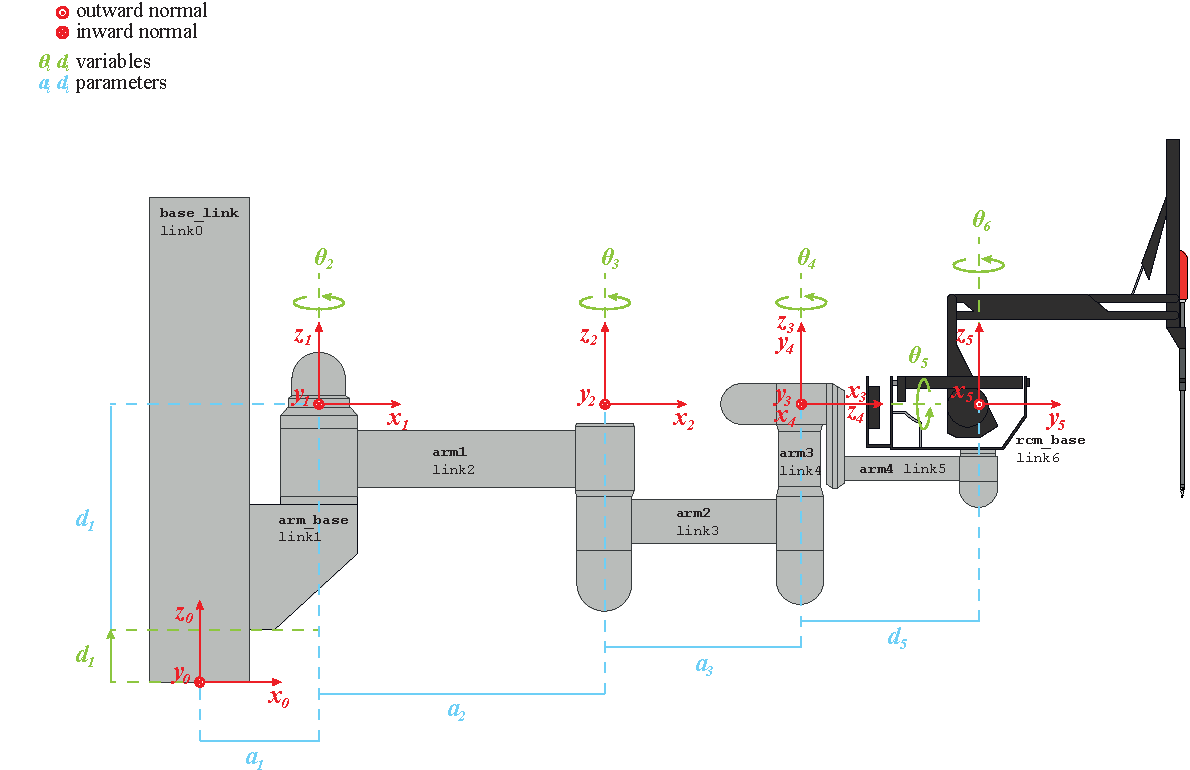
\includegraphics[width=1.1\textwidth]{p4_arm_DH_frames.pdf}\label{fig:p4_arm_DH_frames}}%
	\vspace{5mm}\\
	\hspace*{-15mm}
	\subbottom[Coordinate frames for the joints on the robot hand and instrument.]{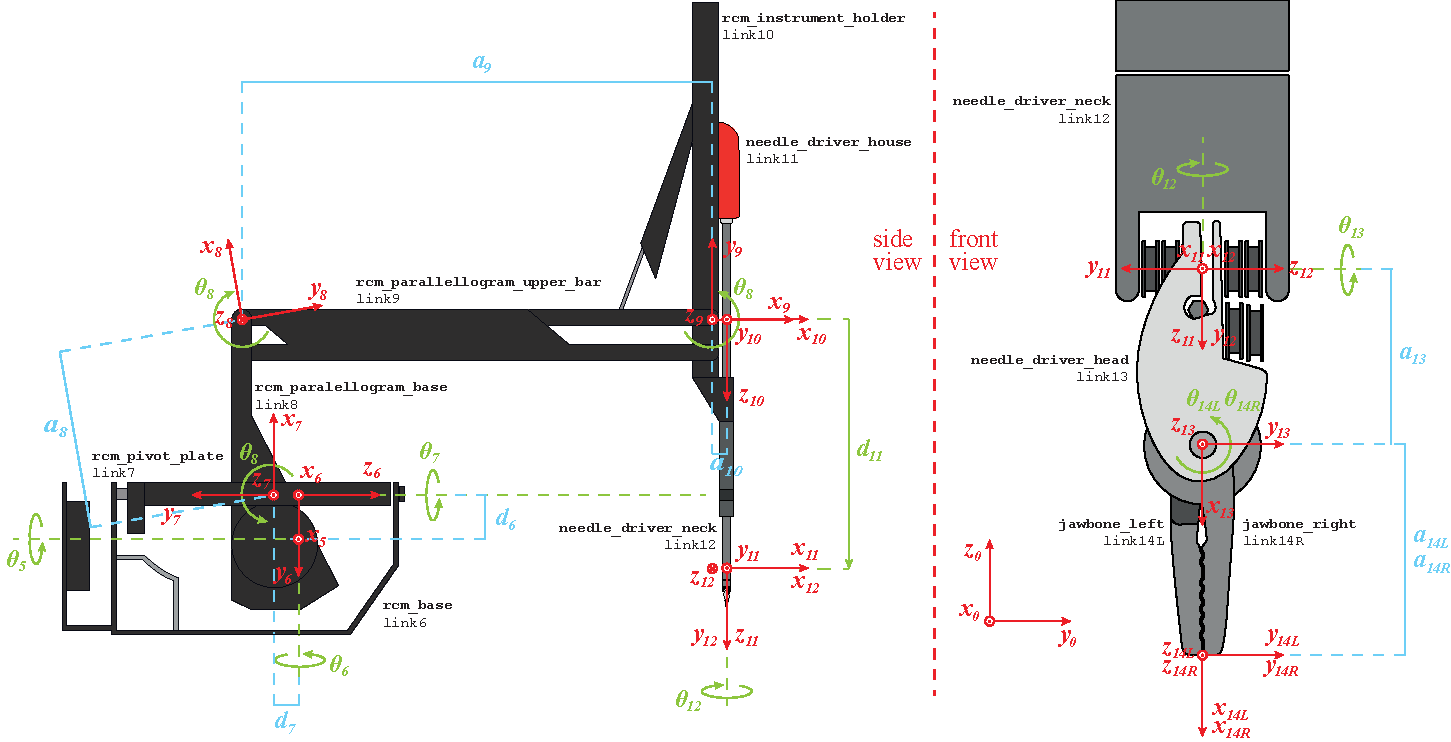
\includegraphics[width=1.15\textwidth]{p4_hand_DH_frames.pdf}\label{fig:p4_hand_DH_frames}}%
	\caption{Orientation and position of coordinate frames $\Psi_0$, $\Psi_b$, $\Psi_1$, ..., $\Psi_{14}$ defined according to the \gls{dh} convention.}
	\label{fig:robot_DH_frames}
\end{figure}

\begin{table}[htbp]
	\small
	\centering
	\begin{tabular}{r | rrrr}\hline
		$i$  & $\theta_i$ [rad]& $d_i$ [m] & $a_i$ [m] & $\alpha_i$ [rad] \\\hline
		1 & 0 &  $0.453+d_1^*$ & 0.198 & 0 \\
		2 & $\theta_2^*$ & 0 & 0.582 & 0 \\
		3 & $\theta_3^*$ & 0 & 0.435 & 0\\
		4 & $\pi/2+\theta_4^*$ & 0 & 0 & $\pi/2$\\
		5 & $\pi+\theta_5^*$ & 0.412 & 0 & $\pi/2$ \\
		6 & $\theta_6^*$ & 0.047 & 0 & $-\pi/2$ \\
		7 & $-\pi/2+\theta_7^*$ & -0.035 & 0 & $-\pi/2$ \\
		8 & $0.03+\theta_8^*$ & 0 & 0.190 & $\pi$ \\
		9 & $0.03+\pi/2+\theta_8^*$ & 0 & 0.515 & $\pi$ \\
		10 & $\theta_8^*$ & 0 & 0.040 & $\pi/2$\\
		11 & 0 & $0.282+d_{11}^*$ & 0  & 0 \\
		12 & $\theta_{12}^*$ & 0 & 0 & $\pi/2$ \\
		13 & $\pi/2+\theta_{13}^*$ & 0 & 0.009 & $\pi/2$ \\
		14L & $\theta_{14L}^*$ & 0 & 0.009 & 0\\
		14R & $\theta_{14R}^*$ & 0 & 0.009 & 0 \\
	\end{tabular}
	\caption{Variables (marked with $^*$) and parameters for the robot in \autoref{fig:robot_DH_frames} defined according to the \gls{dh} convention, where $\theta_i$ and $d_i$ are rotation/translation along $z_{i-1}$, while $a_i$ and $\alpha_i$ are translation/rotation along $x_i$.}
	\label{tab:DH_param}
\end{table}

\subsection{Testing \gls{dh} Kinematics in Matlab}
The new transformation matrices are computed and tested similarly, to determine the accuracy of the defined robot kinematics, and the results are seen in \autoref{tab:DH_distances}.
\begin{lstlisting}[language=matlab]
%% Coordinate frames defined according to Denavit-Hartenberg convention

% Parameters
a_fix = [0.198 0.5820 0.435 0 0 0 0 0.1900 0.515 0.0400 0 0 0.0095 0.0095 0.0095];
d_fix = [1 0 0 0 0.4122 0.0474 -0.0450 0 0 0 0.282 0 0 0 0];
alpha = [0 0 0 pi/2 pi/2 -pi/2 -pi/2 pi pi pi/2 0 pi/2 pi/2 0 0];
theta_fix = [0 0 0 pi/2 pi 0 -pi/2 10/180*pi 10/180*pi+pi/2 0 0 0 pi/2 0 0];

% Variables (signs are included as long as state comes from old frame convention)
d_free = [d1 0 0 0 0 0 0 0 0 0 -d11 0 0 0 0];
theta_free = [0 -th2 -th3 -th4 -th5 th6 th7 th8 th8 th8 0 th12 -th13 th14L -th14R];

% Transformation matrices
for i = 1:length(a_fix)
	Tz = [rot(3,theta_free(i)+theta_fix(i)) [0;0;d_free(i)+d_fix(i)]; zeros(1,3) 1];
	Tx = [rot(1,alpha(i)) [a_fix(i);0;0]; zeros(1,3) 1];
	T_DH(:,:,i) = Tz*Tx;
end
\end{lstlisting}

\begin{table}[htbp]
	\small
\centering
\subbottom[]{%
\begin{tabular}{l r r}\hline
dist. & calc. & meas.\\\hline
$|\,^5_6 p|$ & 4.74 & 5\\
$|\,^5_7 p|$ & 6.54 & 6\\
$|\,^5_8 p|$ & 24.71 & 24\\
$|\,^5_9 p|$ & 49.60 & 49\\
$|\,^5_{10} p|$ & 53.15 & 53\\
$|\,^5_{11} p|$ & 47.94 & 48\\
$|\,^5_{12} p|$ & 47.94 & 48\\
$|\,^5_{13} p|$ & 48.04 & 48\\
$|\,^5_{14} p|$ & 48.16 & 48\\\hline
$\,^0_{14} p_x$ & 210.42 & 210\\
$\,^0_{14} p_z$ & 93.35 & 92
\end{tabular}
\label{tab:state0dh}%
}\hfill
\caption{Calculated and measured distances [cm] between frame origins. In \autoref{tab:state0dh} all variables are set to zero. In \ref{tab:state5dh} state$_\text{hand}=[]$ }
\label{tab:DH_distances}
\end{table}

\textcolor{red}{Add more measurements for verification}





\section{Beating Heart Dynamic Model}
Illustration of heart model and description of kinematics and dynamics.
Quasi-periodic rigid 3D motion, combination of two periodic motions \cite{bib:heart_berkeley}. Frequencies assumed known from ECG and mechanical ventilator.

"The estimated components are then combined to predict future motion of the heart surface. This information, in turn, is used in the design of an explicit controller that stabilizes the relative motion of a surgical tool to a desired distance and orientation with respect to the heart surface."

"We then present a control law that uses the predicted motion to asymptotically stabilize the motion of the surgical tool to a desired distance and orientation with respect to the heart surface."

"To simplify the analysis and allow real-time prediction, we do not take the cause of the motion into consideration, and only consider the kinematics of a local area of interest on the heart surface."

"Fortunately, in this application, we have a reasonably good estimate of the phase1 and frequency of the two motion components: the respiratory phase and frequency can be obtained from the mechanical ventilator, and the cardiac phase and frequency are detected by an ECG monitor."

"choosing a convenient initial position and orientation for $\Psi_d$, e.g. such that $p^d_h(0)=0$ and $R^0_d(0) = I$

Relative configuration between heart and robot tool $H^h_r$ (with $R^h_r =[r_x, r_y, r_z]$) and error function $J(H^h_r)$
\begin{equation}
J(H^h_r) = \underbrace{\tfrac{1}{2}k_p (p^h_r-\Delta r_z)^T(p^h_r-\Delta r_z)}_\text{translational error} + \underbrace{k_x (1-e_x^T r_x) + k_y (1-e_y^T r_y) + k_z (1-e_z^T r_z)}_\text{rotational error}
\end{equation}
\begin{tabular}{rl}
	where &\\
	$\Delta$ & is the desired relative distance between the tool and the heart\\
	$E=[e_x,e_y,e_z]$ & is a rotation matrix describing the desired orientation of the tool frame\\
	$k_p,k_x,k_y,k_z$ & are constant positive parameters\\
\end{tabular}\\

Then $J$ is equal to zero (has its minimum) only when $p^h_r=\Delta r_z$ (the origin of $\Psi_r$ given in h coordinates is $\Delta$ away from the origin of $Psi_h$ along the surface normal) and $R^h_r=E$ (frame h and r axes are aligned).
\begin{align}
\dot{J} &= 
\begin{bmatrix}
k_x \hat{e}_x r_x + k_y \hat{e}_y r_y + k_z \hat{e}_z r_z\\
k_p(p^h_r - \Delta r_z)
\end{bmatrix}^T
\begin{bmatrix}
\omega^{h,h}_r \\
r^{h,h}_r
\end{bmatrix}
= (dJ)^T T^{h,h}_r\\
\dot{H}^h_r &= 
\begin{bmatrix}
\hat{\omega}^{h,h}_r r_x & \hat{\omega}^{h,h}_r r_y & \hat{\omega}^{h,h}_r r_z & \hat{\omega}^{h,h}_r p^h_r + v^{h,h}_r\\
0 & 0 & 0 & 0
\end{bmatrix}\\
(\dot{dJ}) &=
\begin{bmatrix}
-k_x \hat{e}_x \hat{r}_x  - k_y \hat{e}_y \hat{r}_y - k_z \hat{e}_z \hat{r}_z & 0\\
-k_p(\hat{p}^h_r - \Delta \hat{r}_z) & k_p I
\end{bmatrix}
T^{h,h}_r
\end{align}

"We do not consider specific robot dynamics at this point and only specify the desired inertial acceleration $\dot{T}^{0,0}_r$ of the robot end effector frame $\Psi_r$. Proposed desired acceleration"
\begin{equation}
\left(\dot{T}^{0,0}_r\right)_\text{des} = \dot{T}^{0,0}_h - \text{Ad}_{H^0_h} K_1 (\dot{dJ}) + \text{ad}_{T^{0,0}_h} T^{0,h}_r - \text{Ad}_{H^0_h} K_2 (T^{h,h}_r + K_1 dJ)
\end{equation}
\begin{tabular}{rl}
	where & \\
	$K1, K_2$ & are symmetric and positive definite matrices\\
	$H^0_h$ & is the estimated configuration of the frame $\Psi_h$ at the area of interest on the heart surface\\
	$T^{0,0}_h$ & is the estimated velocity of the frame $\Psi_h$ at the area of interest on the heart surface\\
	$\dot{T}^{0,0}_h$ & is the estimated acceleration of the frame $\Psi_h$ at the area of interest on the heart surface\\
\end{tabular}\\

This controller drives $T^{h,h}_r$ to $-K_1dJ$ by the gain $K_2$, along the steepest descend of $J$. Asymptotic stability at $J=0$, with Lyapunov function
\begin{equation}
V=\kappa_1 J + \tfrac{1}{2} (T^{h,h}_r + K_1dJ)^T K_2^{-1}(T^{h,h}_r + K_1dJ)
\end{equation}
\begin{tabular}{rl}
	where & \\
	$\kappa_1$ & is a positive constant strictly less than 4 times the smallest singular value of $K_1$, $0<\kappa_1 <4\sigma_\text{min}(K_1)$
\end{tabular}

Assuming the robot achieves perfect tracking of $\left(\dot{T}^{0,0}_r\right)_\text{des}$, the time derivative of $V$ along the system trajectories is
\begin{equation}
\dot{V} = -\left(T^{h,h}_r + (K_1 - \tfrac{\kappa_1}{2}I)dJ\right)^T \left(T^{h,h}_r + (K_1 - \tfrac{\kappa_1}{2}I)dJ\right) - \kappa_1(dJ ^T(K_1 - \tfrac{\kappa_1}{4}I)dJ
\end{equation}
\begin{tabular}{rl}
	where & \\
	$I$ & is the identity matrix\\
	$K_1 - \tfrac{\kappa_1}{4}$ & is strictly positive because of the choice of $\kappa_1$\\
\end{tabular}